%!TEX root = ../main.tex
\appendix
\appendixpageoff
\section{Threshold correlations on return series}
\label{app:threshold_return}
\begin{figure}[H]
  \caption{Threshold correlations on returns as well as ARMA-GARCH residuals. Page 1/2}
  \label{fig:appendix_threshold1}
  %\toprule
  \centering
  \begin{minipage}{\textwidth}
  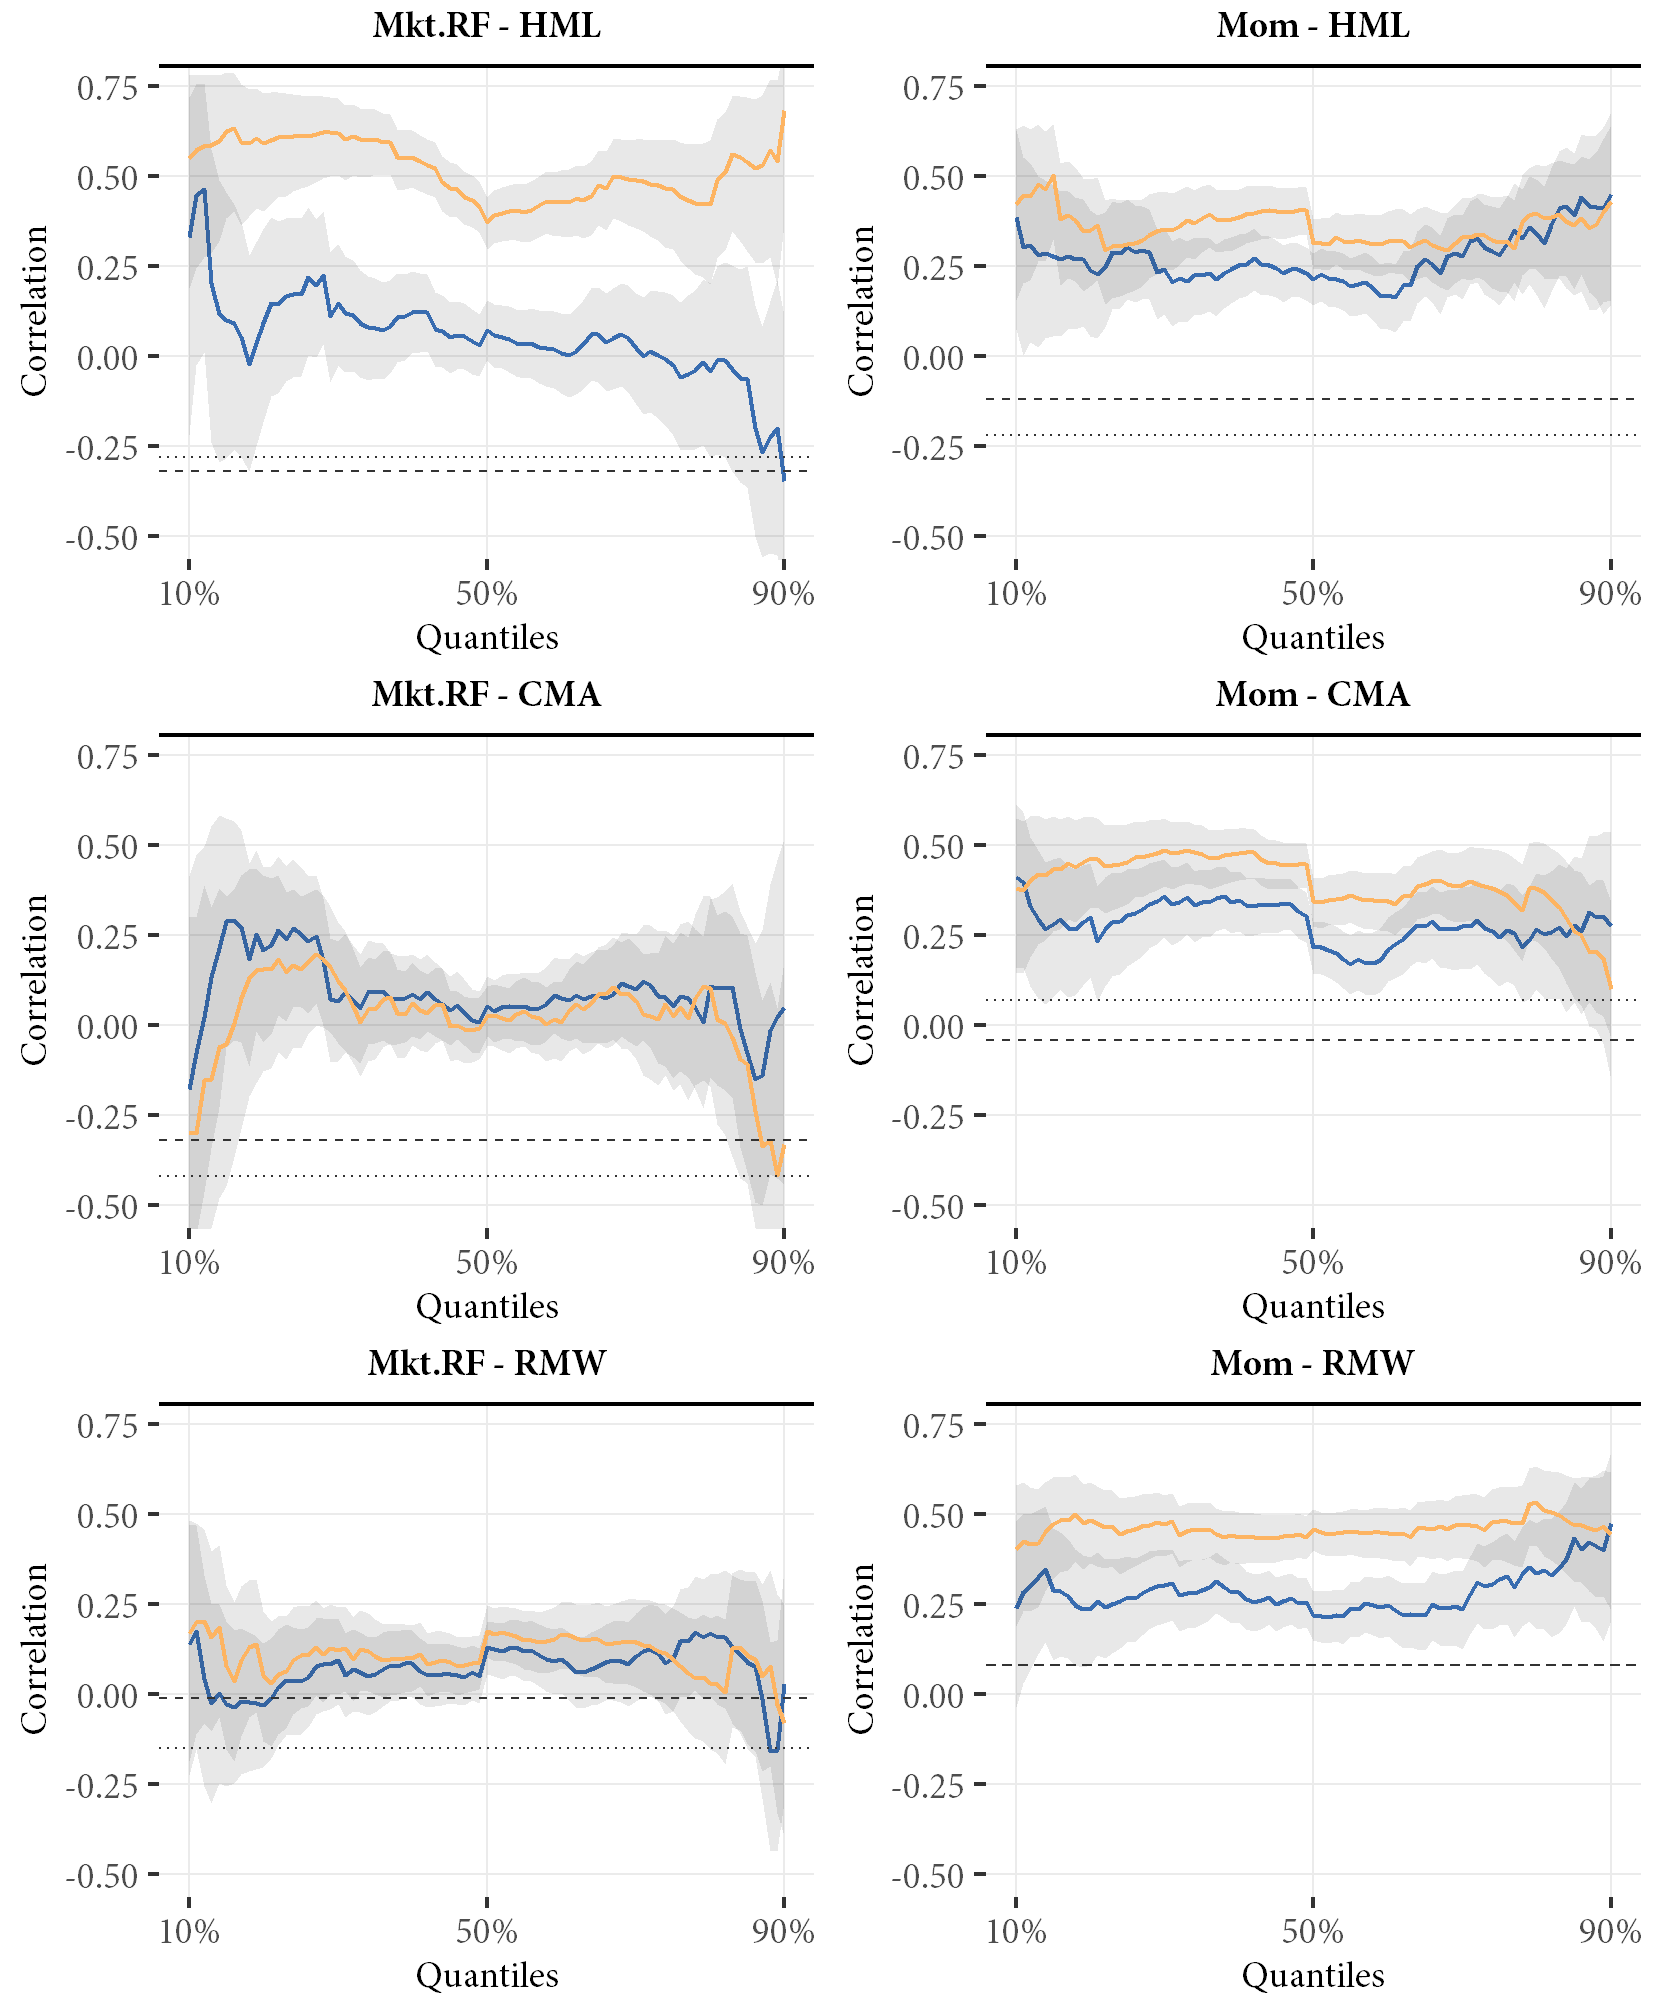
\includegraphics[scale=1]{graphics/appendix_threshold1.png}  
  %\bottomrule
  \vspace{3mm}
  \footnotesize
  Threshold correlation plots with 95\% confidence bounds of both log returns and ARMA-GARCH residuals. Correlation pairs in graph titles. Unconditional correlations on returns and residuals given by the dashed lines. Weekly log returns and ARMA-GARCH residuals from the chosen models, all data 1963-2016
  \end{minipage}
\end{figure}
\begin{figure}[H]
  \caption{Threshold correlations on returns as well as ARMA-GARCH residuals. Page 2/2}
  \label{fig:appendix_threshold2}
  %\toprule
  \centering
  \begin{minipage}{\textwidth}
  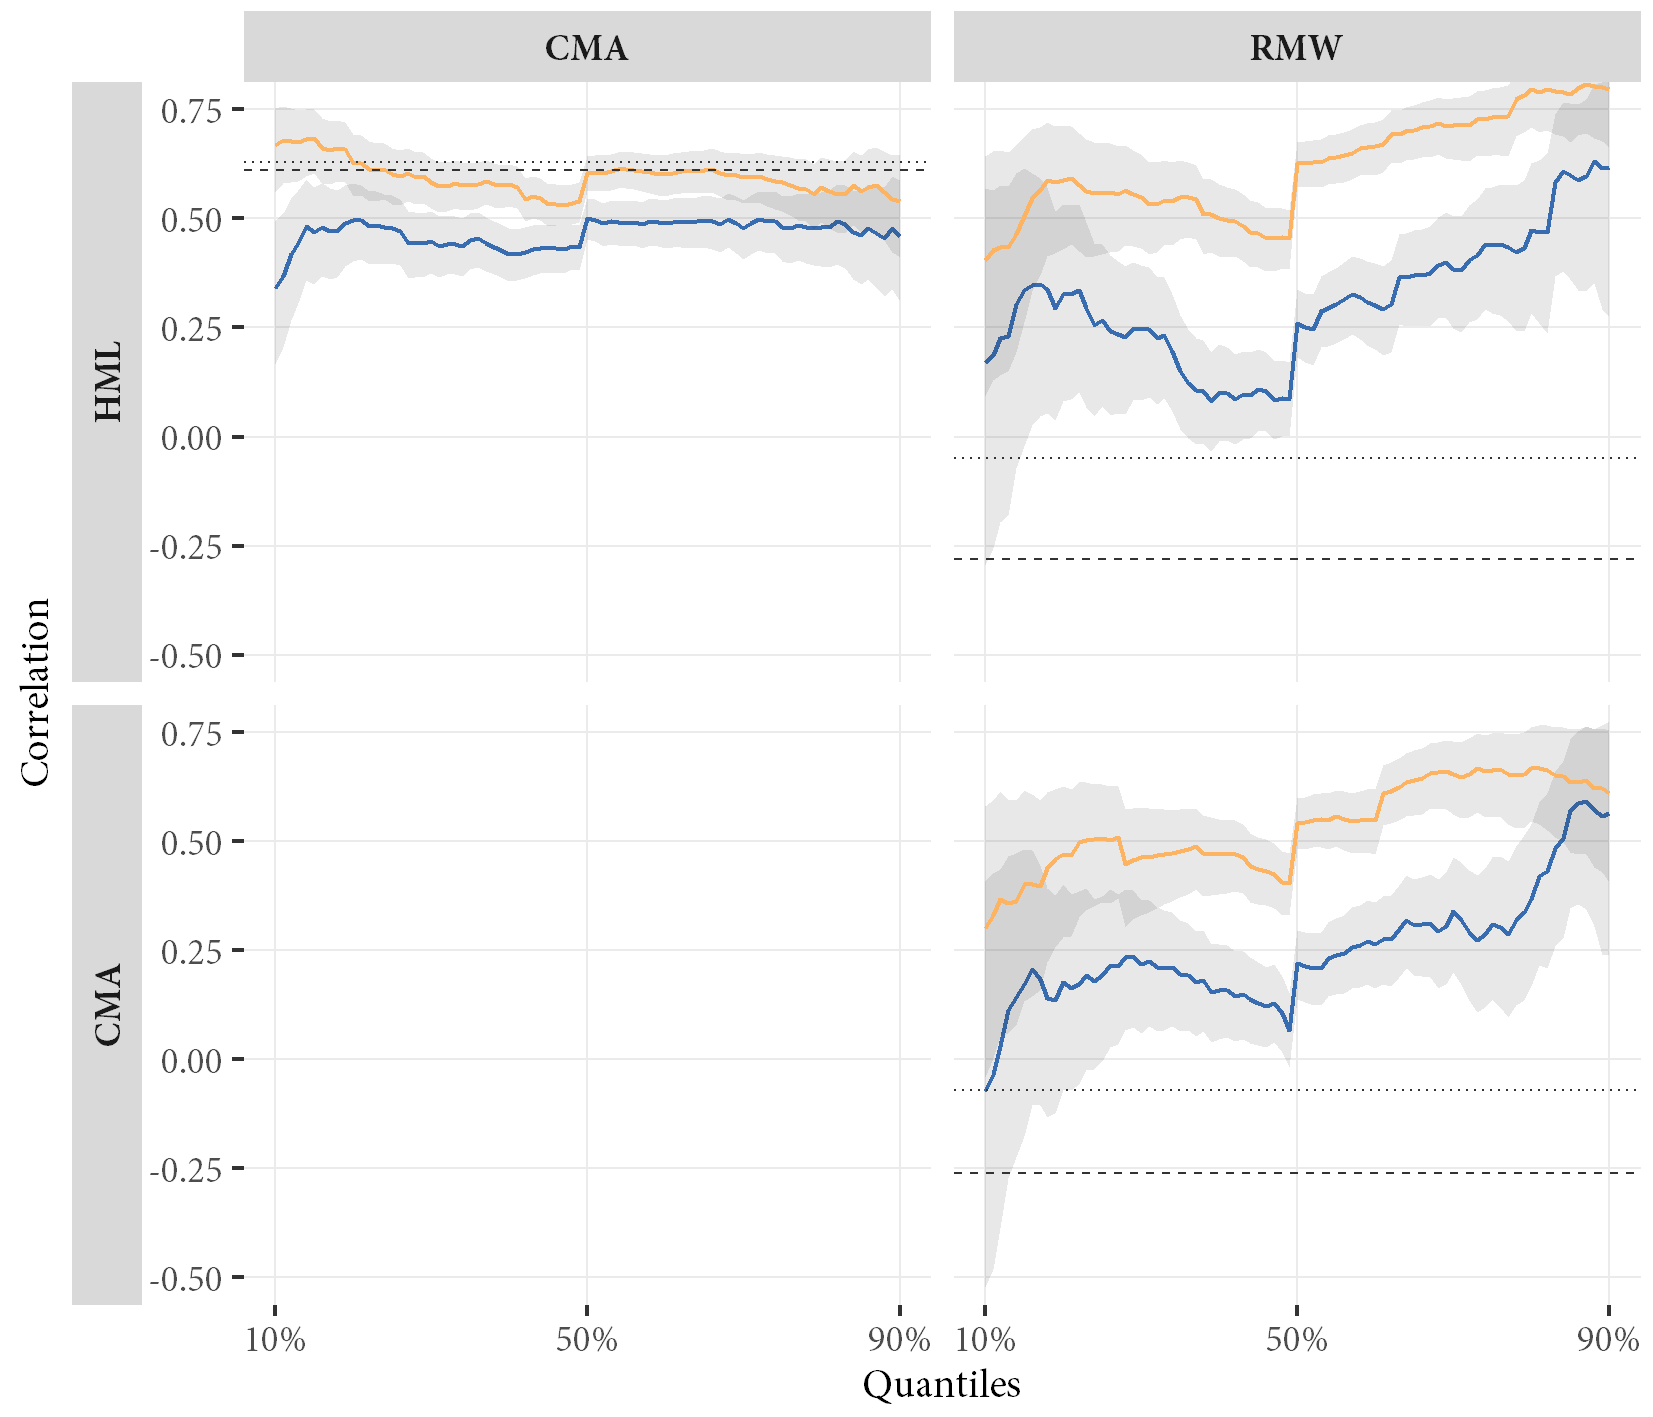
\includegraphics[scale=1]{graphics/appendix_threshold2.png}  
  %\bottomrule
  \vspace{3mm}
  \footnotesize
  Threshold correlation plots with 95\% confidence bounds. Correlation pairs in graph titles. Unconditional correlations on returns and residuals given by the dashed lines. Weekly log returns and ARMA-GARCH residuals from the chosen models, all data 1963-2016
  \end{minipage}
\end{figure}

\newpage

\section{Rolling correlations on return series}
\label{app:rolling_return}
\begin{figure}[H]
  \caption{Rolling correlations on returns as well as ARMA-GARCH residuals. Page 1/2}
  \label{fig:appendix_rolling1}
  %\toprule
  \centering
  \begin{minipage}{\textwidth}
  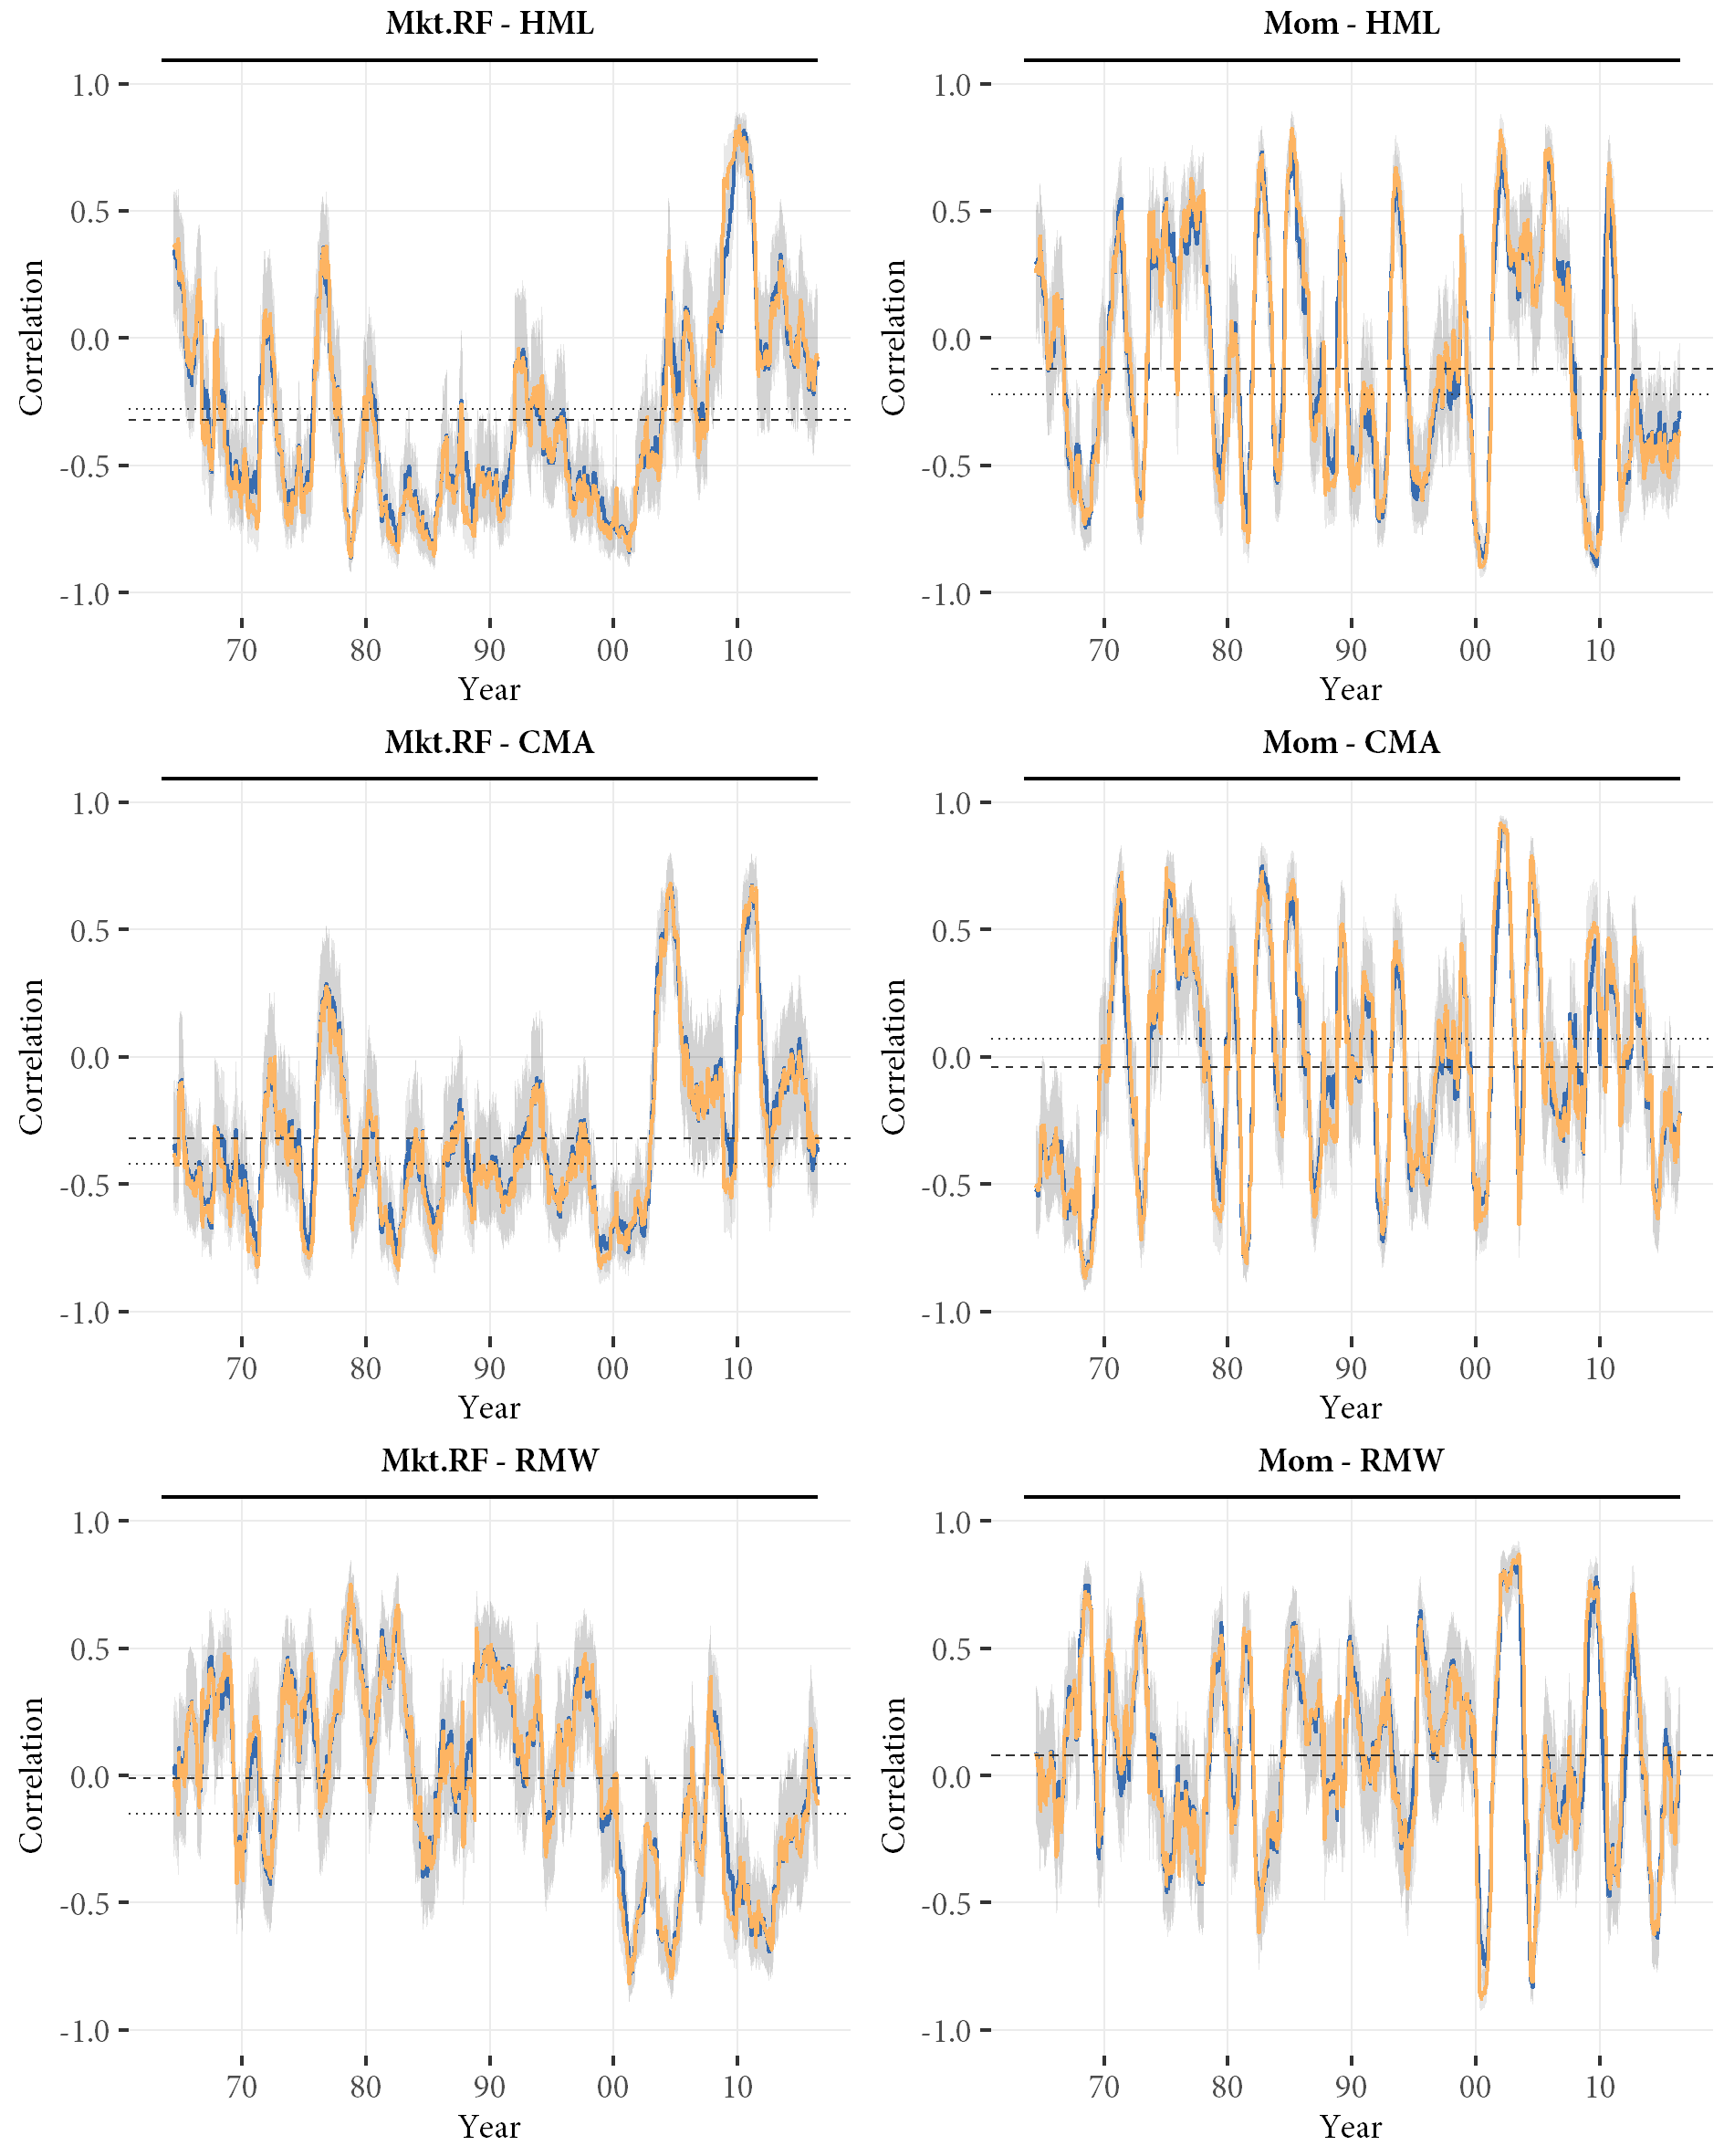
\includegraphics[scale=1]{graphics/appendix_rolling1.png}  
  %\bottomrule
  \vspace{3mm}
  \footnotesize
  Rolling correlation plots with 95\% confidence bounds of both log returns and ARMA-GARCH residuals. Correlation pairs in graph titles. Unconditional correlations on returns and residuals given by the dashed lines. Weekly log returns and ARMA-GARCH residuals from the chosen models, all data 1963-2016
  \end{minipage}
\end{figure}
\begin{figure}[H]
  \caption{Rolling correlations on returns as well as ARMA-GARCH residuals. Page 2/2}
  \label{fig:appendix_rolling2}
  %\toprule
  \centering
  \begin{minipage}{\textwidth}
  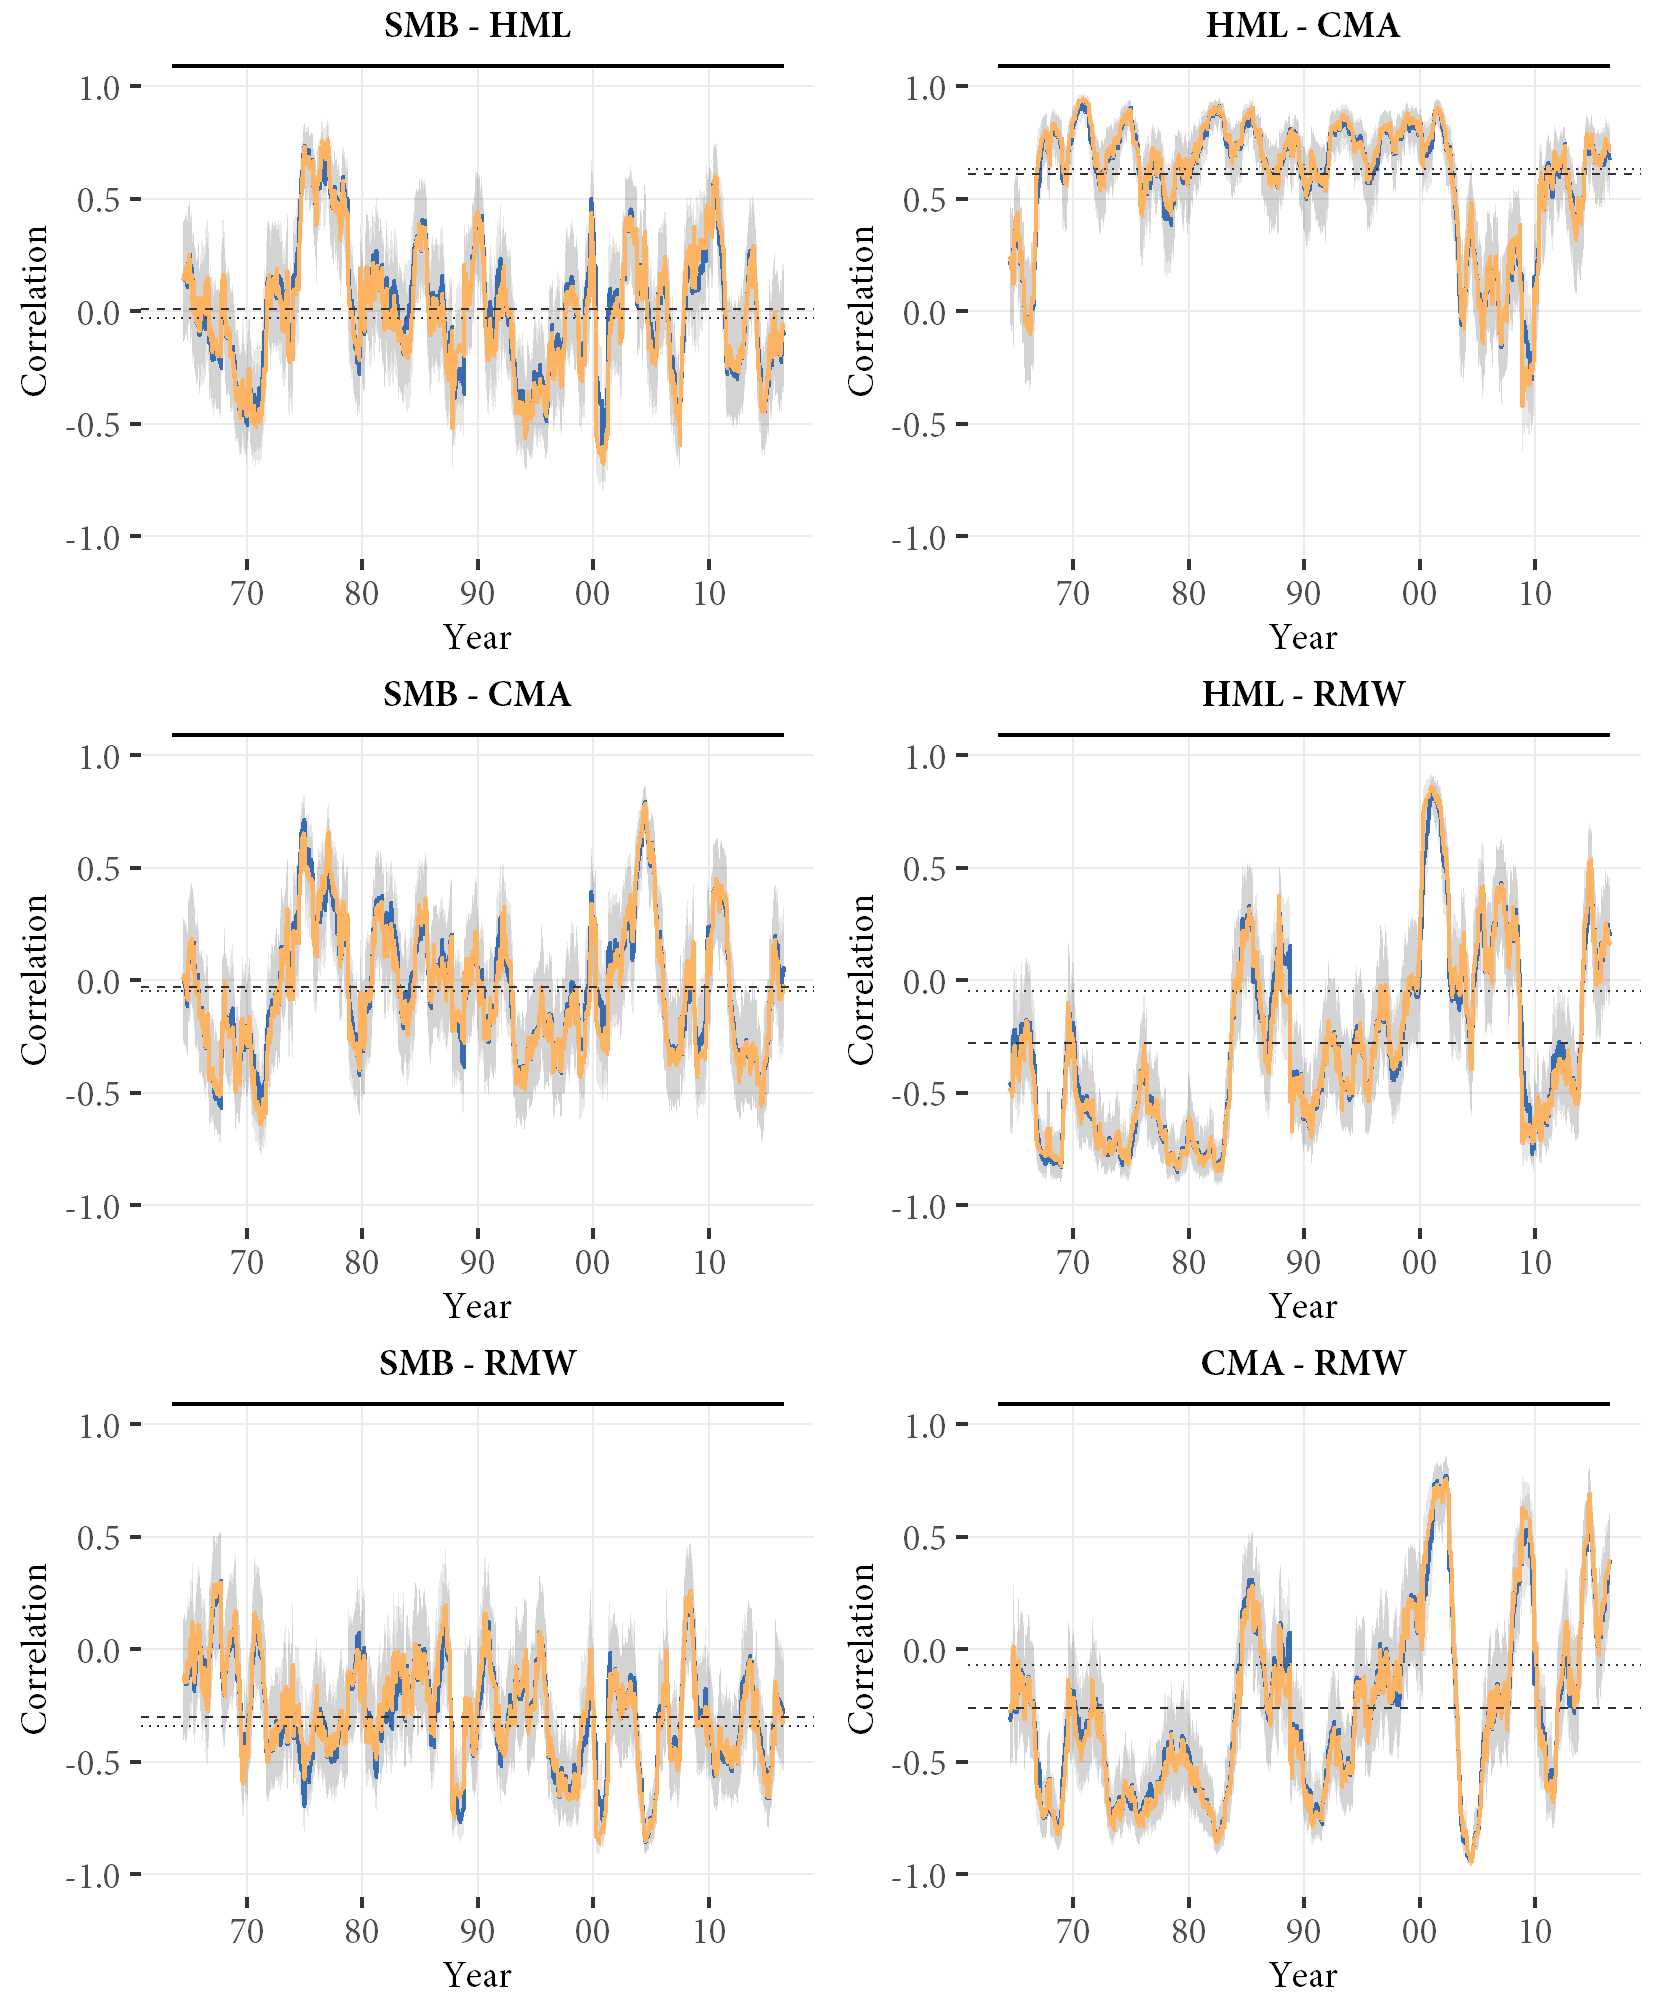
\includegraphics[scale=1]{graphics/appendix_rolling2.png}  
  %\bottomrule
  \vspace{3mm}
  \footnotesize
  Rolling correlation plots with 95\% confidence bounds of both log returns and ARMA-GARCH residuals. Correlation pairs in graph titles. Unconditional correlations on returns and residuals given by the dashed lines. Weekly log returns and ARMA-GARCH residuals from the chosen models, all data 1963-2016
  \end{minipage}
\end{figure}

\newpage

\section{Skewed Student-\textit{t} distribution} 
\label{app:ghstmv}
In line with stylized facts on financial return series, the factor strategies exhibit fat tails and skewness - features that are poorly represented by the normal Gaussian. Our univariate estimations as well as our copula builds on the~\textcite{Hansen1994} skewed Student-\textit{t} distribution. The skewed Student-\textit{t} distribution is, more generally, nested in the generalized hyperbolic distribution~\autocite{McNeilFreyEmbrecht2005}.

The random vector X is distributed multivariate generalized hyperbolic if
\begin{align}
    X \sim \mu + \sqrt{W} A Z + \gamma W
\end{align}
where $\mu$ is the location vector, $\gamma$ is the skewness vector, $R = A A^\top$ is the dispersion matrix, $W$ follows a generalized inverse-gamma distribution $W \sim GIG(\lambda, \chi, \psi)$ and Z is multivariate normal $Z \sim N(\mu^N, R)$, with $W, Z$ independent. The skewed Student-\textit{t} is nested with parameters
\begin{align}
    \lambda = \frac{\nu}{-2} && \chi = \nu - 2 && \psi = 0
\end{align}
where $\nu$ is the degree of freedom. Furthermore
\begin{align}
    \mathbb{E}[X] &= \mu + \mathbb{E}[W] \gamma \\
    Var[X] &= \mathbb{E}[Cov(X|W)] + Cov(\mathbb{E}[X|W]) \\
    &= Var(W) \gamma \gamma^\top + \mathbb{E}[W] R \nonumber
\end{align}
These moments describe the link between the copula correlation matrix $R$ and the skewed Student-\textit{t} distribution's dispersion matrix $R$. Covariances are finite when $\nu > 4$. The multivariate density function is given by
\begin{align} \label{eq:dskewt}
    f_X(x) &= \frac{(\nu - 2)^\frac{\nu}{2} (\gamma^\top R^{-1} \gamma)^{\frac{\nu+d}{2}}}{(2 \pi)^{\frac{d}{2}} |R|^\frac{1}{2} \Gamma (\frac{\nu}{2}) 2^{\frac{\nu}{2} - 1}} \cdot \frac{K_{\frac{\nu + d}{2}} ( \sqrt{(\nu - 2 + Q(x)) \gamma^\top R^{-1} \gamma}) e^{(x-\mu)^\top R^{-1} \gamma} )}{( \sqrt{(\nu - 2 + Q(x)) \gamma^\top R^{-1} \gamma})^{\frac{\nu + d}{2}}}
\end{align}
where $K(\cdot)$ is the modified Bessel function of the second kind, $Q(x) = (x-\mu)^\top R^{-1} (x-\mu)$, $d$ is the length of $x$, and $\Gamma$ is the gamma distribution density.

\newpage

\section{Copula correlation matrix estimation with \textit{c}DCC dynamics} 
\label{app:copula_cdcc}
This is a step-by-step description of the procedure used to find the copula correlation matrix $\{\hat{R_t}\}$ in the \textit{c}DCC case, and has been adapted from \textcite{Aielli2013}.
\begin{enumerate}[(i)]
    \item Re-standardize uniform residuals from univariate ARMA-GJR-GARCH models $\{u_{i}\}$ using the inverse skewed Student-\textit{t} distribution with copula parameters $\nu, \gamma$,  and scale to zero mean and unit variance using the conditional mean and standard deviation\footnote{Unless the copula is normal, the re-standardized residuals $\{\varepsilon^c_i\}$ will not have zero mean and unit variance, which is required for the estimation of the sample correlation matrix $\hat{S}$.}
    \begin{align}
        \varepsilon^c_{i,t} = t^{-1}_{\gamma, \nu}(u_{i,t})
    \end{align}
    \begin{align}
        \varepsilon_{i,t} = \frac{\varepsilon^c_{i, t} - E_{t-1}[\varepsilon^c_{i,t}]}{E_{t-1}[\sigma(\varepsilon^c_{i,t})]}
    \end{align}
    \item Compute the diagonal elements in $Q_t$ over time recursively, initializing with unit diagonal, and using Q-residuals $\{z_i\}$. Utilizing that $\S_{ii} = 1$ (for any correlation matrix), the process for diagonal elements of Q simplifies to
    \begin{align}
        q_{ii, t} &= (1 - \alpha - \beta) + \alpha z_{t-1} z_{t-1}^\top + \beta q_{ii, t-1}
        \intertext{where residuals $\{z_{i}\}$ are initialized at zero and then calculated as}
        z_{i, t} &= \varepsilon_{i, t} \sqrt{q_{ii, t}}
    \end{align}
    \item \label{cdcc:momS} Use Q-standardized residuals $\{z_{i}\}$ to calculate a copula sample correlation matrix
    \begin{align}
        \hat{S} = \frac{1}{T} \sum_{t=1}^{T} z_{t} z_{t}^\top
    \end{align}
    \item Calculate off-diagonal elements of the Q matrix using the copula sample correlation matrix $\hat{S}$ as the long-term correlation matrix in the \textit{c}DCC specification
    \begin{align}
        \hat{Q_t} = (1 - \alpha - \beta) \hat{S} + \alpha z_{t-1} z_{t-1}^\top + \beta Q_{t-1}
    \end{align}
    \item Standardize $\hat{Q_t}$ to the copula correlation matrix $\hat{R_t}$ and calculate the sum of log-likelihoods for a given parameter set $\Theta = \{\nu, \gamma, \alpha, \beta\}$
\end{enumerate}
% \subsection{Exogenous regressors in copula cDCC}
% It is relatively straightforward to make $S$ time-varying by adding a time-varying component $\Upsilon_t$ to it. Following the general case of~\autocite{ChristoffersenErrunzaJacobLanglois2012}, $\Upsilon_t$ is constructed from an $N\times(N + N_X)$ matrix $A$ where $N$ is the number of factors, and $N_X$ the number of explanatory variables. With the $N \times N_X$ matrix of coefficients $\theta$ and explanatory variables $X$, construct $A$ from an $NxN$ identity matrix and the element-wise multiplications of $\theta$ and $X$:
% \begin{align}
%   A &=
%     \begin{bmatrix}
%     1 & 0 & \cdots & 0            & \quad & \theta_{11} X_{11,t} & \cdots & \theta_{1N_X} X_{1N_X,t} \\
%     0 & 1 & \cdots & 0            & \quad & \theta_{21} X_{21,t} & \cdots & \theta_{2N_X} X_{2N_X,t} \\
%     \vdots & \vdots & \ddots & 0  & \quad & \vdots &               \vdots & \vdots \\
%     0 & 0 & \cdots & 1            & \quad & \theta_{N1} X_{N1,t} & \cdots & \theta_{NN_X} X_{NN_X,t}
%     \end{bmatrix}
% \end{align}
% Normalize $A$ by dividing each element with the root mean square of its row to ensure $\Upsilon_t$ is a correlation matrix:
% \begin{align}
%   \bar{A}_{ij} &= \frac{A_{ij}}{\sqrt{\sum_{k = 1}^{N + N_X} A_{ik}^2}}
% \end{align}
% Finally,
% \begin{align}
%   \Upsilon_t &= \bar{A} \bar{A}^\top
% \end{align}
% It is now straightforward to let e.g. $X_{ij} = t$ for a time-trend, or any other independent variable, common or asset specific. The new time-invariant component $\Omega$ should be estimated based on the sample averages of both the standardized shocks and $\Upsilon_t$. Replacing~\autoref{cdcc:momS} in the above list, we estimate $\hat{\Omega}$ as:
% \begin{align}
%   \hat{\Omega} &=
%     \frac{
%       \frac{1}{T} \sum^{T} z_t z_t^\top -
%       \phi
%       \frac{1}{T} \sum^{T} \Upsilon_t
%     }{1 - \phi}
% \end{align}

\newpage

\section{Stationary bootstrap of copula parameter standard errors} \label{App:Appendix_bootstrap}
We rely on the multi-step maximum likelihood estimation of the copula model, which takes the standardized residuals of marginal distributions as given in the second step. The first estimation step introduces parameter uncertainty that is not taken into account by the conventional standard errors of the second estimation.\footnote{Here, our model deviates from~\textcite{ChristoffersenLanglois2013}, who use a semi-parametric model that uses the empirical density function, and find standard errors using the analytical approach in~\textcite{ChenFan2006}. However, those errors are not valid in a time-varying copula context, as the estimation of means and variances impact the asymptotic distributions of copula parameters~\autocite{Remillard2010}.} We use the stationary block bootstrap method of \textcite{PolitisRomano1994} with a block length of 45 weeks (approx. 1 year of data) to find reliable standard errors for copula parameters. The procedure is theoretically supported by \textcite{GonclavesWhite2004} and implemented as follows:
\begin{enumerate}[(i)]
    \item Generate a block bootstrap version of the original weekly return data
    \item Estimate the ARMA-GJR-GARCH models and calculate standardized residuals
    \item Transform standardized residuals to uniform and estimate the copula model
    \item Collect the copula parameters $\Theta_i$
    \item Repeat (i)-(iv) N times to get $\{\Theta_i\}^{N}_{i=1}$
    \item Use the standard errors from the empirical distribution of $\{\Theta_i\}^{N}_{i=1}$
\end{enumerate}

\newpage

\section{Univariate diagnostic tests}
\label{app:univariate_diagnostics}

\textbf{Autocorrelation test}

The autocorrelation test is a weighted Ljung-Box test, following~\textcite{FisherGallagher2012} and~\textcite{LjungBox1978}. Under the null of a correctly specified model with no serial correlation, the weighted Ljung-Box test has been shown to generate results closer to its asymptotic distribution than the standard Ljung-Box test. The test statistic is given by
\begin{align}
  Q_W = T (T+2) \sum\limits^m_{k = 1} \frac{m-k+1}{m} \frac{\hat{r}_{k}^{2} (\hat{\epsilon}_{t} / \hat{\sigma}_{t})}{T-k}
\end{align}
where $T$ is the number of observations, $\hat{r}^{2}_{k} ( \hat{\epsilon}_{t} / \hat{\sigma}_{t} )$ is the squared sample autocorrelation of standardized residuals with lag order $k$ and max lag order $m$. Under the null, the test statistic is asymptotically distributed $\sum\limits^m_{k = 1} \chi^2_k \gamma_k$, where $\{\chi^2_k\}$ are independent chi-squared random variables with one degree of freedom and $\{\gamma_k\}$ are eigenvalues of a weighting matrix. We consider two maximum lag orders, 5 and 10 weeks. The maximum lag length was chosen by visual inspection of the autocorrelation functions for standardized residuals.

\textbf{Volatility clustering test}

For ARCH effects, we use the weighted LM test, following~\textcite{FisherGallagher2012} and~\textcite{LiMak1994}. The test has the null of no autocorrelation in standardized squared residuals from the model, and the test statistic is given by:
\begin{align}
  LM_W = T \sum\limits_{k = b + 1}^{m} \frac{m - k + (b+1)}{m} \hat{r}^{2}_{k} (\hat{\epsilon}^{2}_{t} / \hat{\sigma}_{t})
\end{align}
where $T$ is the number of observations, $b$ the number of autoregressive lags in the GARCH ($b=1$), $\hat{r}^2_k (\hat{\epsilon}^2_t / \hat{\sigma}_t)$ is the squared sample autocorrelation of standardized squared residuals with lag order $k$ and max lag order $m$. Under the null, the test statistic is asymptotically distributed $\sum\limits^m_{k = 1} \chi^2_k w_k$, where $\{\chi^2_k\}$ are independent chi-squared random variables with one degree of freedom and $\{w_k\}$ are the weighting parameters ($w = (m - k + (b+1))/m$). The maximum lag length was chosen by visual inspection of the autocorrelation functions for standardized squared residuals.

\textbf{Leverage effect test}

We use the sign bias test of~\textcite{EngleNg1993} to determine whether there are significant leverage effects in the factor returns. Run the regression
\begin{align}
  \hat{z}_t^2 = c_0 + c_1 I_{\hat{\epsilon}_{t-1} < 0} + c_2 I_{\hat{\epsilon}_{t-1} < 0} \cdot \hat{\epsilon}_{t-1} + c_3 I_{\hat{\epsilon}_{t-1} \geq 0} \cdot \hat{\epsilon}_{t-1} + u_t
\end{align}
where $\hat{z}_t^2$ are the standardized squared residuals of the ARMA-GARCH model, $I_\cdot$ are indicator functions that are equal to one when the subscript conditions are true, and $\hat{\epsilon}_{t-1}$ are the lagged ARMA-GARCH residuals. For the test of negative sign bias (i.e. leverage effect), the null hypothesis is $H_0: c_2 = 0$, and for the test of positive sign bias (i.e. reverse leverage effect), the null hypothesis is $H_0: c_3 = 3$. The Wald test statistics are asymptotically distributed $\chi^2$ with one degree of freedom.


